\documentclass[aspectratio=169]{beamer}
\setbeameroption{show notes}

\usepackage{beamerthemeVT}
\usepackage{graphicx} % Load images
\usepackage{booktabs}

\usepackage[style=ieee, backend=biber]{biblatex}
\addbibresource{references.bib}

\title{3D Radio Environment Map Modeling for Aerial Wireless Networks}
\subtitle{Ryan Frost\\Advisor: Dr. Liu\\Collaborators: Shadab \& Dr. Haihan}
\author{Ryan Frost}
\date{\today}

\begin{document}

\begin{frame}
	\titlepage
\end{frame}

\begin{frame}{Background}
	\begin{columns}
		\begin{column}{0.5\textwidth}
			\begin{itemize}
				\setlength\itemsep{1em}
				\item M.Eng. in CPE Candidate
				\item B.S. in Engineering from JMU
				\item \textbf{Interest Areas:}
				      \begin{itemize}
					      \setlength\itemsep{0.5em}
					      \item Embedded Systems
					      \item Cyber-Physical Systems
					      \item Edge Machine Learning
				      \end{itemize}
			\end{itemize}
		\end{column}
		\begin{column}{0.5\textwidth}
			\begin{figure}
				\centering
				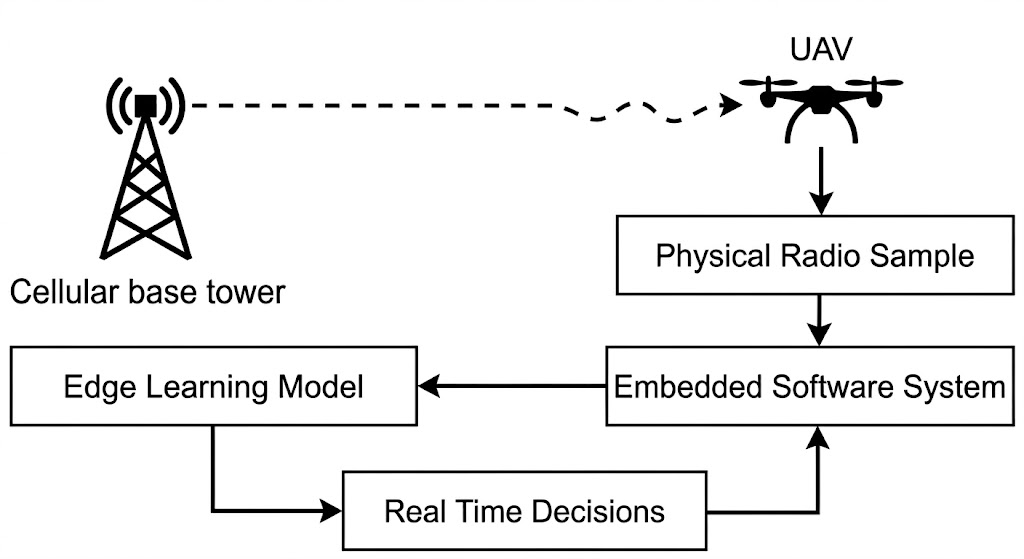
\includegraphics[width=1\textwidth, keepaspectratio]{CyberPhysicalDiagram.jpeg}
				\caption{Cyber-Physical UAV Integrated System}
			\end{figure}
		\end{column}
	\end{columns}

	\note{Here is a quick background on me.
		I'm a Masters of Engineering in Computer Engineering Candidate here at Virginia Tech.
		I have a Bachelor's of Science in Engineering from JMU.
		My intereset areas are embedded systems, cyber-physical systems, and edge machine learning.
		I'm interested not only in where physics meets software, but also how we can leverage light weight learning models to make decisions on those physical measurements without access to unlimited compute resources.
		This led me to pursue Dr.
		Liu's research team where I've had the opportunity to research the role Unmanned Aerial Vehicles (UAVs) play in quickly deploying wireless networks in unique scenarios.
	}
\end{frame}

\begin{frame}{Research Space}
	\begin{columns}
		\begin{column}{0.5\textwidth}
			\begin{itemize}
				\setlength\itemsep{1em}
				\item Why are UAVs being used for wireless networks?
				\item \textbf{Scenarios:}
				      \begin{itemize}
					      \setlength\itemsep{0.5em}
					      \item Disaster relief
					      \item Remote areas
					      \item Tactical operations
				      \end{itemize}
			\end{itemize}
		\end{column}
		\begin{column}{0.5\textwidth}
			\begin{figure}
				\centering
				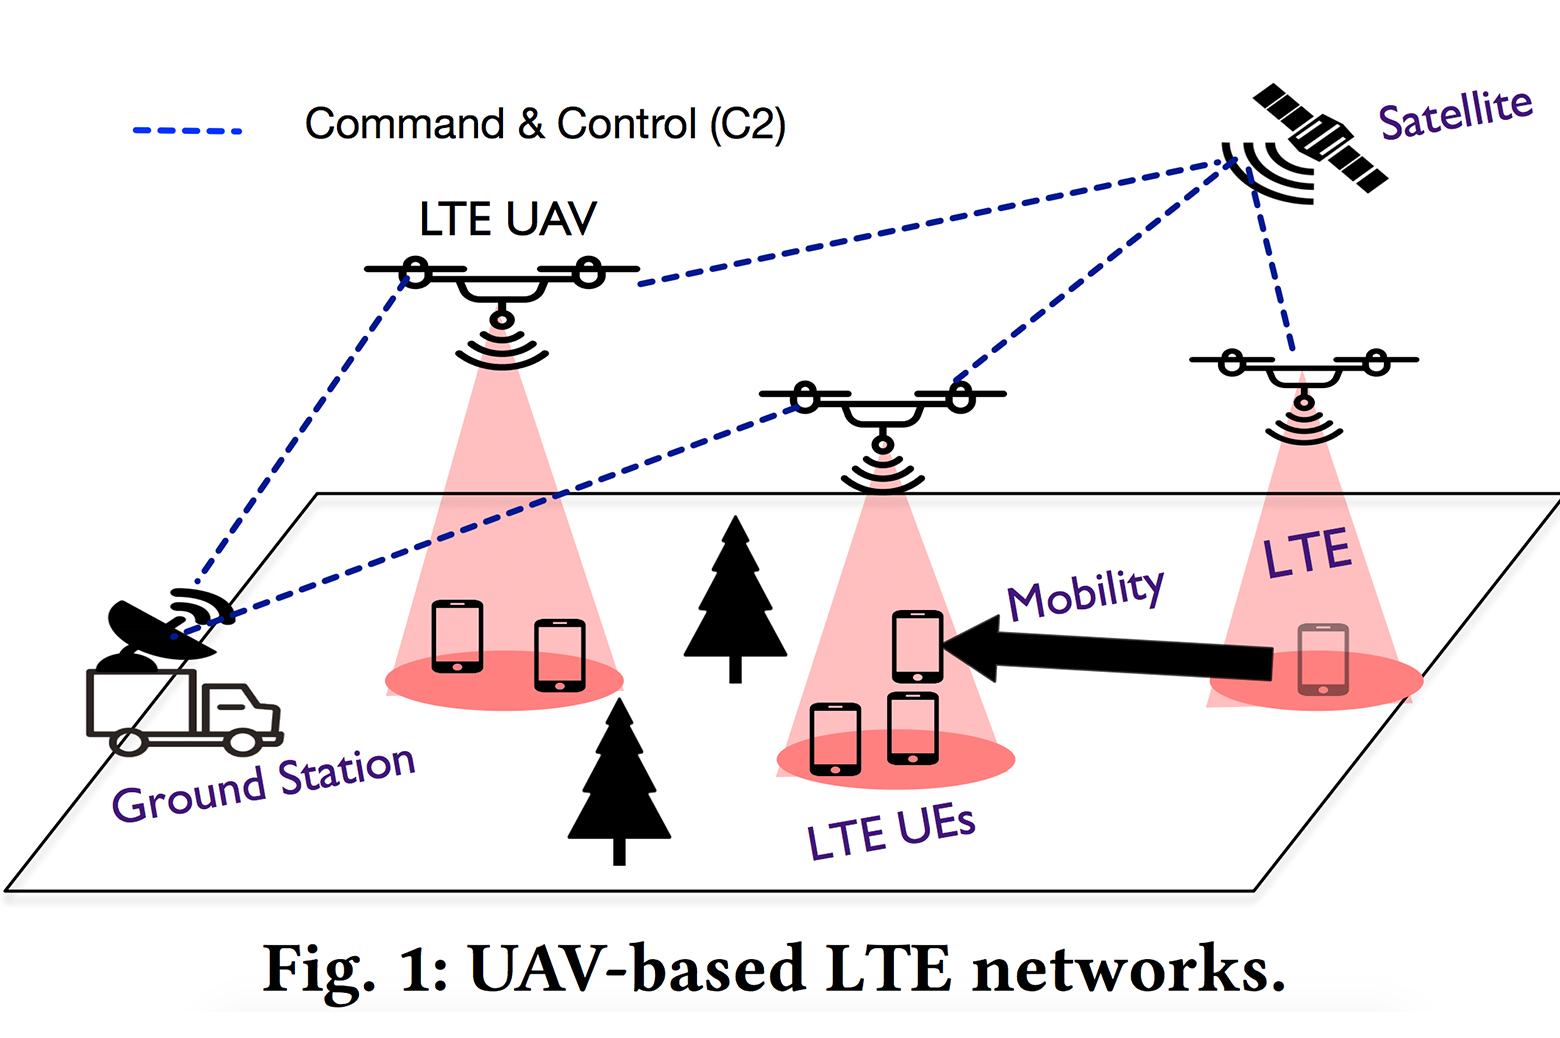
\includegraphics[trim={0 5cm 0 0}, clip, width=1\textwidth, keepaspectratio]{UAV_Integration.jpg}
				\caption{UAV-supported Command \& Control Network \cite{b1}}
			\end{figure}
		\end{column}
	\end{columns}

	\note{To set the foundation of the project, it is important to understand why UAVs are being used for wireless networks.
		As it turns out, they are very useful for rapidly deploying aerial base stations when the usual grounded base station infrastructure is either destroyed or non existent.
		Example scenarios include disaster relief, remote areas of the planet, and tactical operations.
		Advances in UAV technology has allowed for this innovation in wireless networks, and this is a wide area of research sponsored by private companies and the government alike.
	}
\end{frame}

\begin{frame}{Problem Space}
	\begin{columns}
		\begin{column}{0.5\textwidth}
			\begin{itemize}
				\setlength\itemsep{1em}
				\item How do we provide connection to the widest area using UAVs?
				\item \textbf{Challenges:}
				      \begin{itemize}
					      \setlength\itemsep{0.5em}
					      \item Varying altitude adds new dimension
					      \item Limited sample size
					      \item Limited power and compute on UAV
				      \end{itemize}
			\end{itemize}
		\end{column}
		\begin{column}{0.5\textwidth}
			\begin{figure}
				\centering
				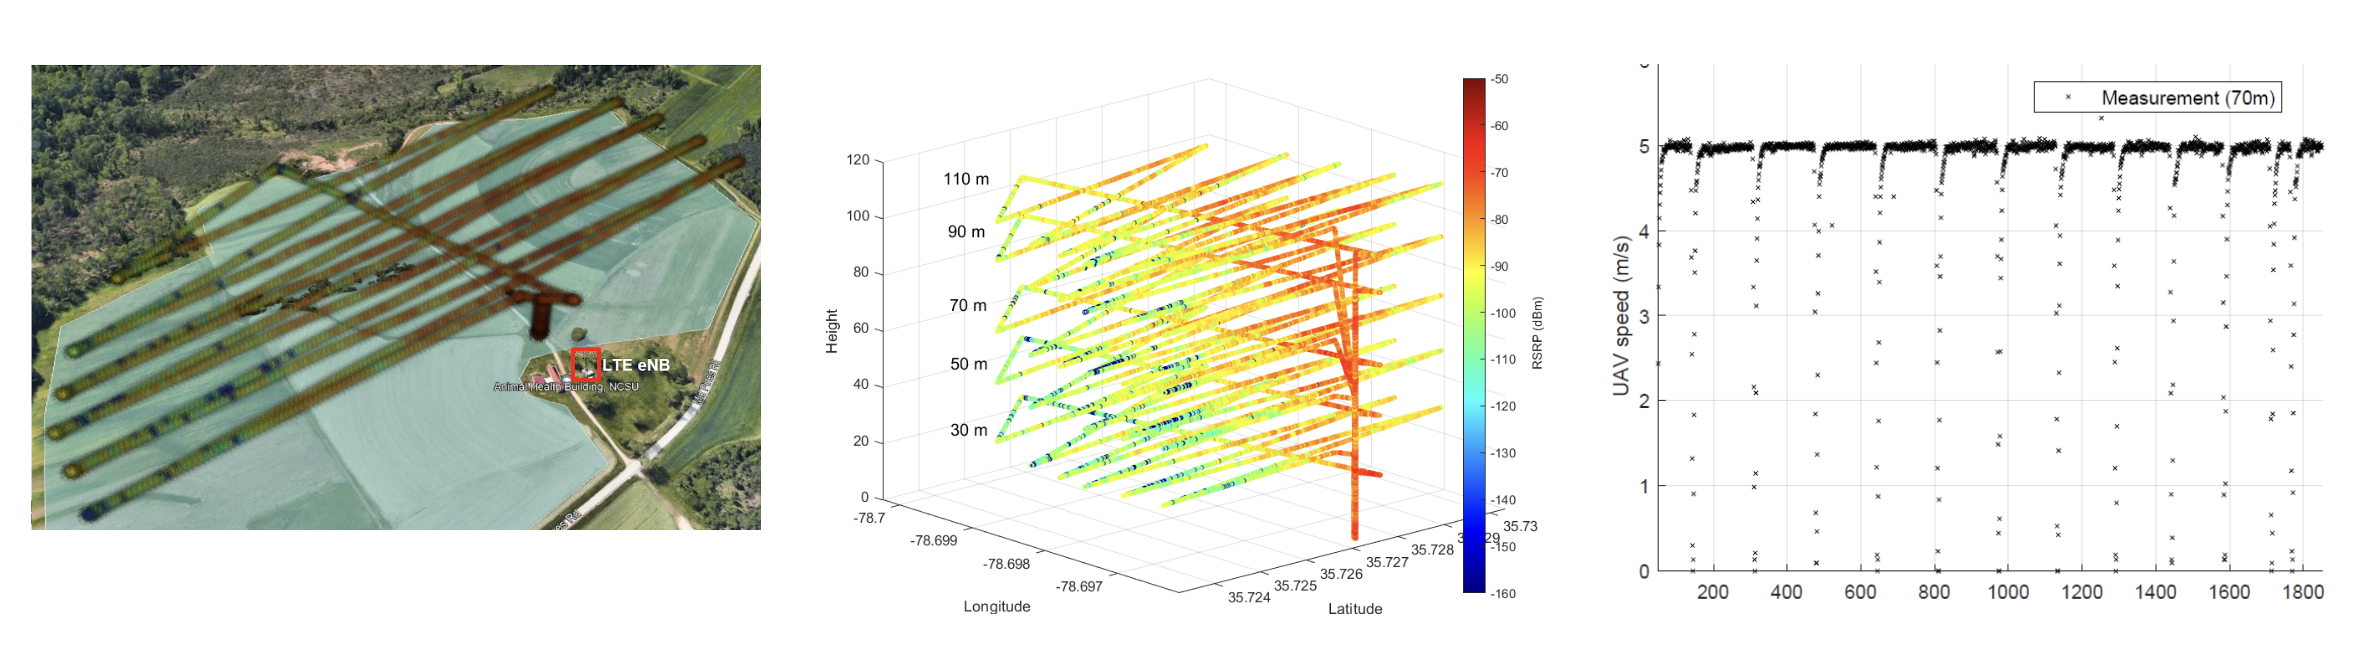
\includegraphics[trim={14cm 0 14cm 0}, clip, width=0.9\textwidth, keepaspectratio]{UAV_Altitudes.png}
				\caption{3D Environment Map Sampling using UAV \cite{b2}}
			\end{figure}
		\end{column}
	\end{columns}

	\note{The natural next question to ask when setting up a UAV-based wireless network is how do we provide connection to the widest area with the resources we have? This question poses its own unique challenges for aerial networks beyond the established ground-based networks. The most obvious challenge is the varying altitude of UAVs. We now want to understand connectivity in 3 dimesions to know where to position our UAVs. Not only do we add a new dimension, but based on the scenarios described earlier, we are working in areas that have little to no radio map data. Disasters will change the connectivity landscape, and remote areas and tactical operations will inherintly have little to no prior data. That is on top of collecting samples in a whole new dimension, making samples even more sparse. Additionally, we don't have the power supply of a ground base station, which means limited real-time compute on the UAV itself. This is the problem space the my project works in.}
\end{frame}

\begin{frame}{Project Layout}
	\begin{columns}
		\begin{column}{0.5\textwidth}
			\begin{itemize}
				\setlength\itemsep{1em}
				\item 5 Month Timeframe
				\item \textbf{Phases:}
				      \begin{enumerate}
					      \setlength\itemsep{0.5em}
					      \item Analyze existing AERPAW datasets
					      \item Develop dataset processing pipeline
					      \item Develop machine learning pipeline
					      \item Explore extreme learning machine
				      \end{enumerate}
			\end{itemize}
		\end{column}
		\begin{column}{0.5\textwidth}
			\begin{figure}
				\centering
				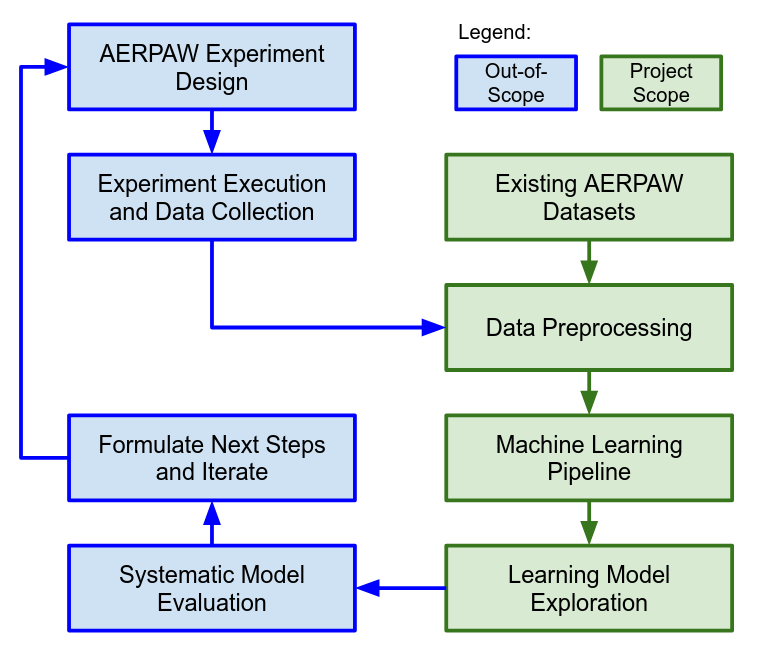
\includegraphics[width=0.9\textwidth, keepaspectratio]{Layout_Flowchart.png}
				\caption{Project Layout Flowchart}
			\end{figure}
		\end{column}
	\end{columns}

	\note{Given the problem space, I worked with Dr. Liu's student Shadab as well as Dr. Haihan to establish a 5 month project that would be both a standalone exploration of the problem space and serve as a starting point for future research. Our starting point was NC State's Aerial Experimentation and Research Platform for Advanced Wireless, hence known as AERPAW. They have a number of published datasets from UAV flights with RSRP samples and a single base station. For this project, we downselected the published datasets and selected a few to work with. Then I worked on a dataset processing pipeline to evaluate the suitability of selected datasets. I also created a machine learning pipeline that builds on the processing pipeline to feed the data into learning models. Finally I explored the viability of an extreme learning model compared to baseline models for in-flight real-time training and inference.}
\end{frame}

\begin{frame}{Phase 1: AERPAW Dataset Analysis}
	\begin{columns}
		\begin{column}{0.27\textwidth}
			\begin{itemize}
				\setlength\itemsep{1em}
				\item AERPAW vs

				      Digital Twin
				\item \textbf{Dataset Criteria:}
				      \begin{itemize}
					      \setlength\itemsep{0.5em}
					      \item UAV-based
					      \item 3D trajectory
					      \item RSRP values
				      \end{itemize}
			\end{itemize}
		\end{column}
		\begin{column}{0.73\textwidth}
			\begin{figure}
				\centering
				\raisebox{12pt}{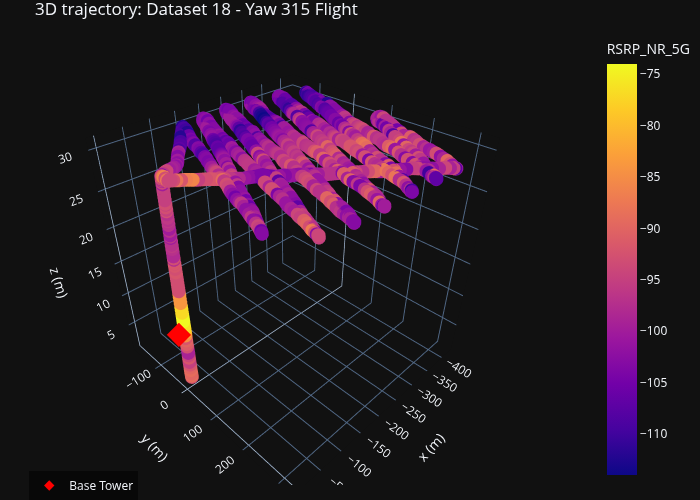
\includegraphics[width=0.42\textwidth, keepaspectratio]{dataset_18_Yaw_315_Flight_3d.png}}
				\raisebox{15pt}{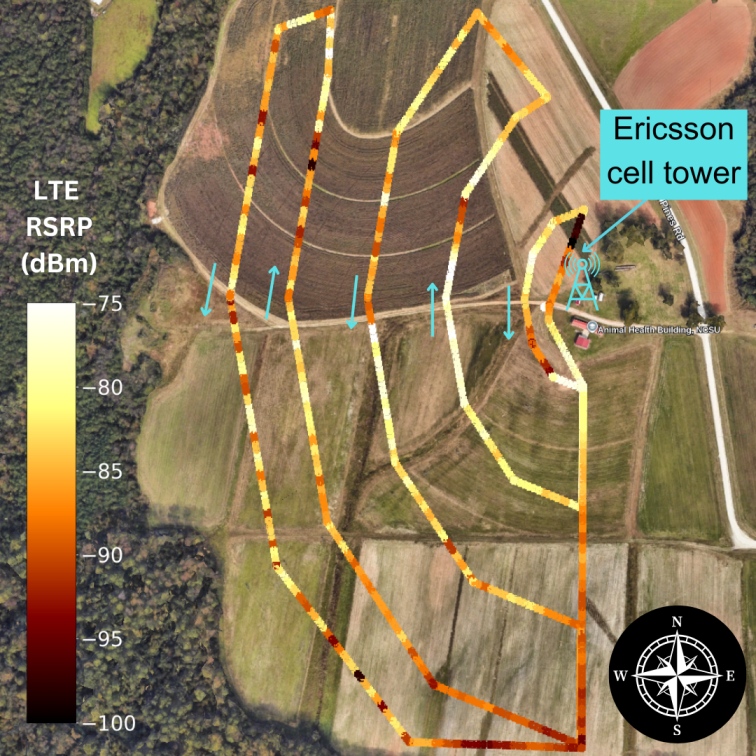
\includegraphics[width=0.29\textwidth, keepaspectratio]{dataset22trajectory.jpg}}
				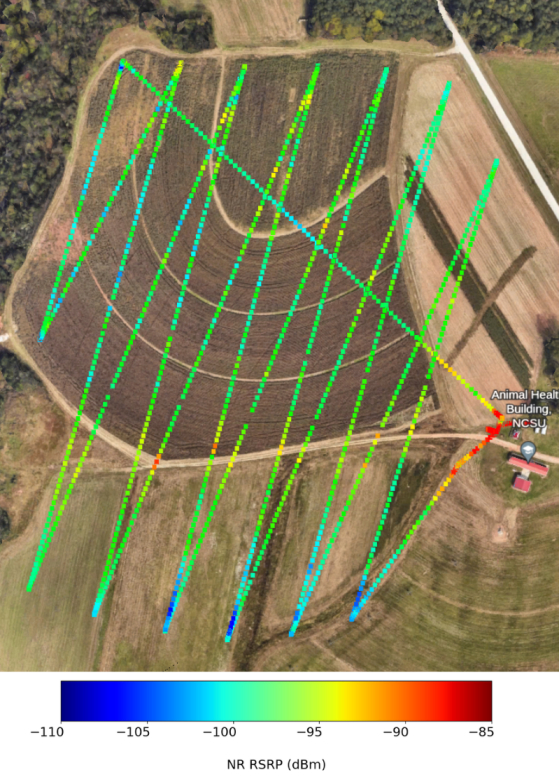
\includegraphics[width=0.25\textwidth, keepaspectratio]{dataset24trajectory.jpg}
				\caption{UAV Trajectory for Datasets 18, 22 \cite{b3}, 24 \cite{b4}}
			\end{figure}
			\small
			\resizebox{\textwidth}{!}{%
				\begin{tabular}{cccc}
					\toprule
					\textbf{Number of Flights} & \textbf{Total Samples} & \textbf{Avg Timestep} & \textbf{Avg Distance} \\
					\midrule
					11                         & 9927                   & $\sim$1s              & 5 - 10m               \\
					\bottomrule
				\end{tabular}%
			}
		\end{column}
	\end{columns}

	\note{To briefly explain AERPAW, AERPAW is a platform where a researcher can program an experiment virtually and schedule it to be run on NC State's drone field testbed. This is very useful for real world, repeatable data collection. But why would we need real world data when there are already existing digital twin-based simulated radio environment maps? Well, simluated environments lack the nuances and fluctuations that exist in real-world scenarios, and those fluctuations act as crucial features for a learning model to train on. I then had to analyze the 28 published datasets based on three criteria: the dataset had to be UAV-based with a 3D trajectory and recorded RSRP values. Based on this, the team selected datasets 18, 22, and 24 for further analysis.}
\end{frame}

\begin{frame}{Phase 2: Data Processing Pipeline}
	\begin{columns}
		\begin{column}{0.5\textwidth}
			\vspace{0.3cm}
			\begin{itemize}
				\setlength\itemsep{1em}
				\item Medain Absolute Deviation (MAD)
				\item Spatial Correlation
				\item Fast-Fading Correlation
			\end{itemize}
			\begin{figure}
				\centering
				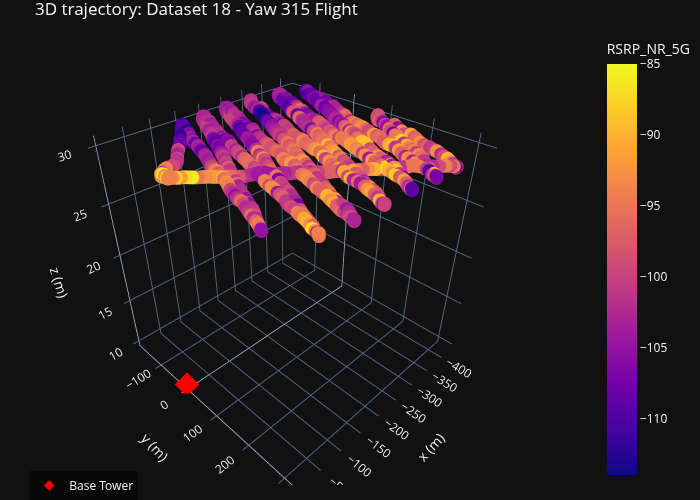
\includegraphics[width=0.6\textwidth, keepaspectratio]{dataset_18_Yaw_315_Flight_mad_3d.png}
				\caption{MAD Filtering of Dataset 18 Trajectory}
			\end{figure}
		\end{column}
		\begin{column}{0.5\textwidth}
			\begin{figure}
				\centering
				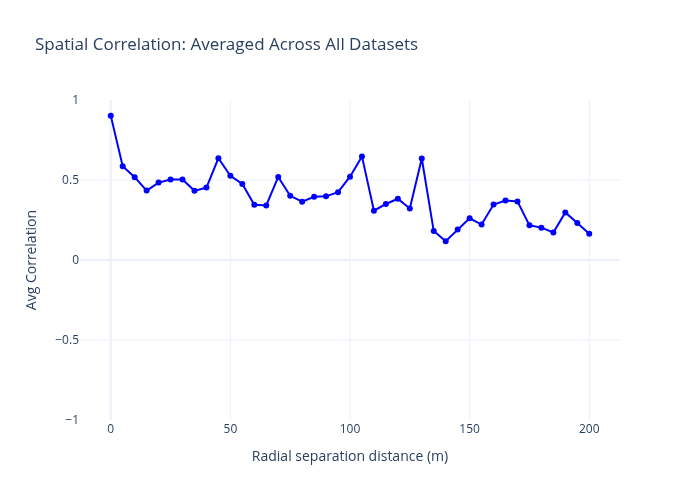
\includegraphics[trim={0 0 0 1cm}, clip, width=0.75\textwidth, keepaspectratio]{all_datasets_spatial_correlation_avg.png}
				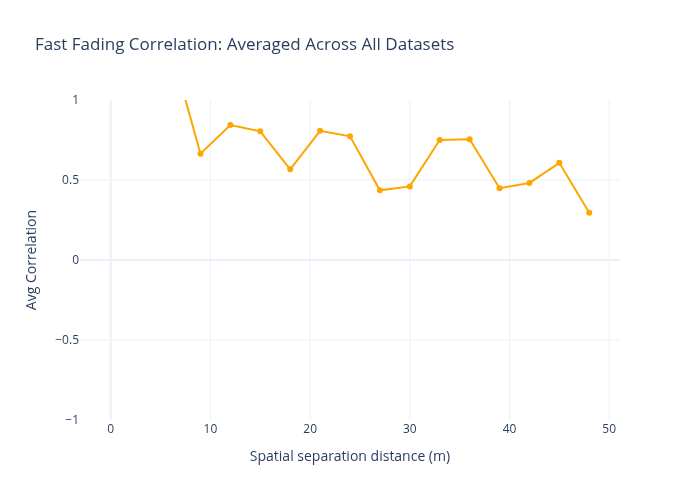
\includegraphics[trim={0 0 0 1cm}, clip, width=0.75\textwidth, keepaspectratio]{all_datasets_ff_correlation_avg.png}
			\end{figure}
		\end{column}
	\end{columns}

	\note{The first step in using the datasets was converting them all to the same format. One useful processing technique was taking the medain altitude to remove the UAV ascent and descent. This was done to focus on the variation in RSRP at further distances. To better understand how RSRP values change with space and time, a spatial correaltion and fast-fading correlation analyses were performed. At this point, we were mimicing some very recent work by folks at NC State (Gautham Reddy, Kursat Tekbıyık, Bryton Petersen, Antoine Lesage-Landry, Gunes Karabulut Kurt, and Ismail Guvenc). The spatial correlation shows how datapoints that are close in space have higher correlation within the same region. The fast-fading correlation shows how datapoints that are close in both space and time have higher correlation, although the sample-to-sample RSRP has greater variation than the region-based analysis likely due to to changing line of sight conditions. Essentially, we are identifiying the opportuinity for a learning model to actually learn.}
\end{frame}

\begin{frame}{Phase 3: Machine Learning Pipeline}
	\begin{columns}
		\begin{column}{0.5\textwidth}
			\begin{itemize}
				\setlength\itemsep{1em}
				\item Line of Sight Path Loss
				      \begin{itemize}
					      \item RSME: 17.4918 dB
				      \end{itemize}
				\item PyTorch Dataloader
				\item InceptionTime
			\end{itemize}
			\vspace{1cm}
			$$ FSPL = (\frac{4\pi df}{c})^{2}$$
			\centering
			\scriptsize
			\color{VTOrange} \textbf{Eq. 1:}
			\color{black} Line of Sight Path Loss \\ (d = distance, f = frequency, c = speed of light)
		\end{column}
		\begin{column}{0.5\textwidth}
			\begin{figure}
				\centering
				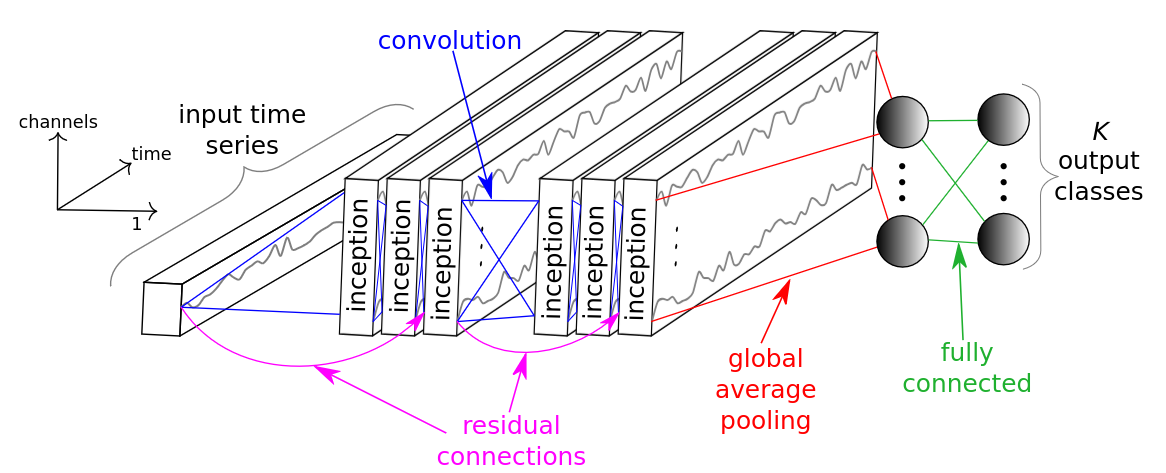
\includegraphics[width=1\textwidth, keepaspectratio]{InceptionModel.png}
				\caption{Inception Network for Time Series Classification \cite{b5}}
			\end{figure}
			\small
			\resizebox{\textwidth}{!}{%
				\begin{tabular}{cccccc}
					\toprule
					\textbf{Train \%} & \textbf{Val \%} & \textbf{Test \%} & \textbf{Epochs} & \textbf{Test RSME} & \textbf{Train Time} \\
					\midrule
					0.7               & 0.15            & 0.15             & 100             & 3.6468 dB          & 577.36s             \\
					\bottomrule
				\end{tabular}%
			}
		\end{column}
	\end{columns}

	\note{After analyzing the correlation features, I modeled the Radio Enviornment Map using Line of Sight Path Loss,
		which essentially predicts signal strength in ideal conditions when you have line of sight.
		For these datasets, it falls short with a very high RSME of 17.4918 dB.
		Then I implemented an established deep learning model called Inception.
		It is typically used for image processing but can be modified for time series data.
		This performed much better, with an RSME of 3.6468 after 100 epochs, although returns were marginal
		after just 50 epochs.
		The result of this phase was confirmation that we can better model the Radio Environment Map with
		established deep learning methods.
	}
\end{frame}

\begin{frame}{Phase 4: Extreme Learning Machine}
	\begin{columns}
		\begin{column}{0.3\textwidth}
			\begin{itemize}
				\setlength\itemsep{1em}
				\item Limited Sample Analysis
				\item Limited Compute Analysis
			\end{itemize}
		\end{column}
		\begin{column}{0.7\textwidth}
			\begin{columns}[onlytextwidth]
				\begin{column}{0.4\textwidth}
					\begin{figure}
						\centering
						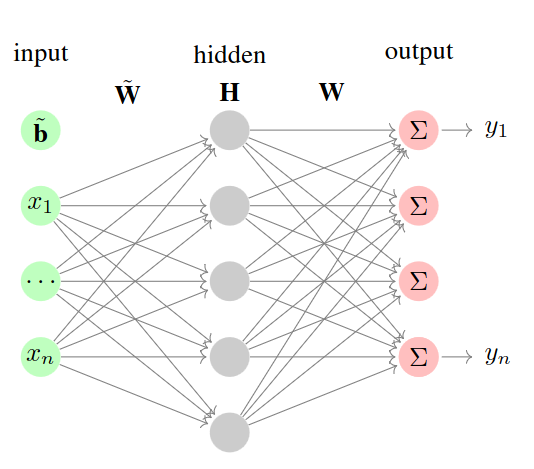
\includegraphics[width=\textwidth, keepaspectratio]{elm_model.png}
						\caption{Extreme Learning Machine Model \cite{b6}}
					\end{figure}
				\end{column}

				\begin{column}{0.48\textwidth}
					$$f(x) = \sum_{i=1}^{L} \beta_i g(w_i \cdot x + b_i)$$
					{
							\centering
							\scriptsize
							\color{VTOrange} \textbf{Eq. 2:}
							\color{black} General single-hidden layer feedfoward network (SLFN) equation \\
						}
						{
							\tiny
							\vspace{0.1cm}
							$w_i$ = wieght vector input to node $i$ \\
							$b_i$ = bias of node $i$ \\
							$\beta_i$ = trained ouptut weight \\
						}
					$$\hat{\beta} = H^\dagger T$$
					\centering
					\scriptsize
					\color{VTOrange} \textbf{Eq. 3:}
					\color{black} Moore-Penrose generalized inverse optimization
					\vspace{0.1cm}

				\end{column}
			\end{columns}
			\small
			\resizebox{\textwidth}{!}{%
				\begin{tabular}{cccccc}
					\toprule
					\textbf{Samples} & \textbf{Inception RSME} & \textbf{ELM RSME} & \textbf{Inception Train Time} & \textbf{ELM Fit Time} & \textbf{Inception Epochs} \\
					\midrule
					100              & 4.1208 dB               & 7.7501 dB         & 66.25s                        & 0.0950s               & 38                        \\
					500              & 3.7646 dB               & 4.1769 dB         & 75.26s                        & 0.1517s               & 38                        \\
					1000             & 4.1965 dB               & 3.9045 dB         & 66.14s                        & 0.4981s               & 29                        \\
					2000             & 5.0473 dB               & 3.7208 dB         & 62.89s                        & 3.5166s               & 22                        \\
					6948             & 4.2300 dB               & 3.8771 dB         & 74.30s                        & 2.2450s               & 13                        \\
					\bottomrule
				\end{tabular}%
			}
		\end{column}
	\end{columns}

	\note{The next phase was to push beyond just the baselines and implement an Exteme Learning Machine.
		This lightweight model relies on a random hidden layer and only trains on the output weights from
		the hidden layer to the output layer.
		This simplification removes expensive back propagation and replaces it with a simple linear time fit function
		called the Moore-Penrose generalized inverse optimization.
		As we established earlier, for a quick deployment in a new area, the limited number of samples and limited access
		to heavy compute resources makes large deep learning models difficult to utilize.
		I perfomed a limited sample training of the Inception and Extreme Learning Machine models to show how
		RSME and training time compares.
		Inception runs for about 60 seconds regardless of the sample size because when there are a smaller number of
		samples, it takes longer to train to reach our set threshold of 5 RSME.
		ELM fits much faster and also has better performance at all sample levels.
	}
\end{frame}

\begin{frame}{Phase 4: Extreme Learning Machine}
	\begin{columns}
		\begin{column}{0.5\textwidth}
			\small
			\resizebox{\textwidth}{!}{%
				\begin{tabular}{ccccccc}
					\toprule
					\% Train & Inc RMSE & ELM RMSE & Inc Train (s) & ELM Fit (s) & Inc Inf (ms) & ELM Inf (ms) \\
					\midrule
					20\%     & 97.0953  & 37.9405  & 1.87          & 0.0333      & 0.3427       & 0.2165       \\
					40\%     & 85.6834  & 12.7268  & 3.74          & 0.0670      & 0.3585       & 0.2259       \\
					60\%     & 93.3388  & 5.8723   & 5.61          & 0.0977      & 0.3788       & 0.2295       \\
					80\%     & 28.9217  & 5.1637   & 7.49          & 0.1520      & 0.4784       & 0.2551       \\
					\bottomrule
				\end{tabular}%
			}
			\\
			\vspace{0.2cm}
			\centering
			{\scriptsize Specific Flight: Dataset\_24\_PawPrints\_5G\_30m\_Flight\_2.csv}

			\vspace{1cm}

			\small
			\resizebox{\textwidth}{!}{%
				\begin{tabular}{ccccccc}
					\toprule
					\% Train & Inc RMSE & ELM RMSE & Inc Train (s) & ELM Fit (s) & Inc Inf (ms) & ELM Inf (ms) \\
					\midrule
					20\%     & 92.4061  & 29.9600  & 4.44          & 0.0873      & 0.3370       & 0.2190       \\
					40\%     & 78.4127  & 11.0304  & 8.62          & 1.0688      & 0.3503       & 0.2304       \\
					60\%     & 67.9661  & 4.9897   & 12.84         & 1.1330      & 0.3556       & 0.2257       \\
					80\%     & 27.0395  & 4.7115   & 17.05         & 2.0811      & 0.3860       & 0.2411       \\
					\bottomrule
				\end{tabular}%
			}
			\\
			\vspace{0.2cm}
			{\scriptsize All Flights Averaged}
		\end{column}
		\begin{column}{0.5\textwidth}
			\begin{figure}
				\centering
				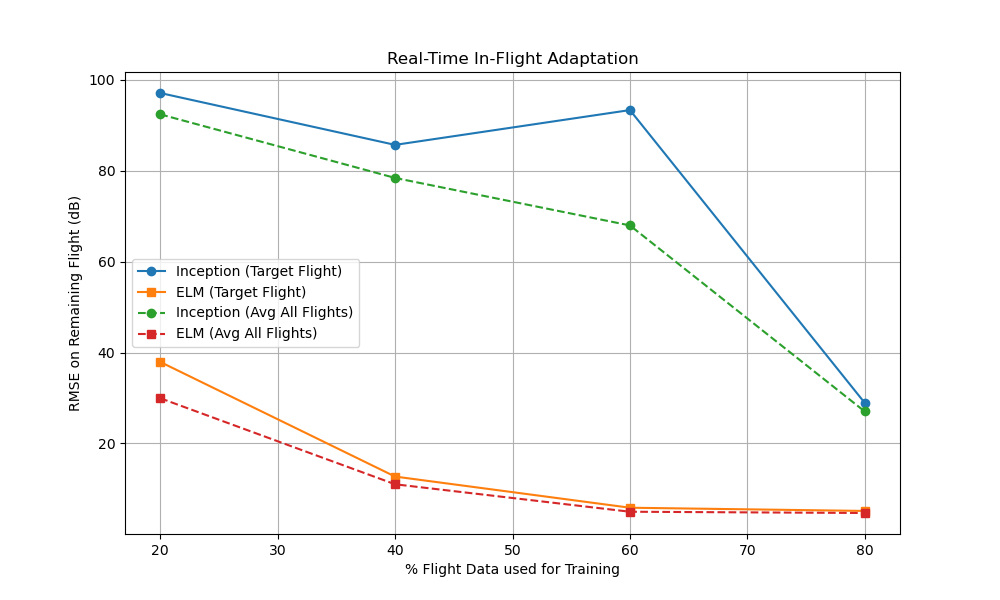
\includegraphics[width=\textwidth, keepaspectratio]{real_time_simulation.png}
				\caption{Real-Time In-Flight Learning}
			\end{figure}
		\end{column}
	\end{columns}

	\note{To emulate a real-world scenario, I trained the models at specific points throughout each individual flight.
		At 20\%, 40\%, 60\%, and 80\% both models would train and be tested on the rest of the unseen flight.
		This proved highly effective in showing the usefulness of the ELM model under very limited sample sizes, and the
		performance was reasonable for the extrapolated data.
		The graph on the right shows how as the flight progresses, ELM is much faster at learning than Inception, and
		for a single flight, is almost always more accurate.
	}
\end{frame}

\begin{frame}{Discussion \& Conclusion}
	\begin{columns}
		\begin{column}{0.5\textwidth}
			\begin{itemize}
				\setlength\itemsep{1em}
				\item What if we had a much larger sample size from roughly the same time?
				\item At what point does a deep learning model surpass a light wieght model?
				\item What useful metrics could be collected in a real-world test?
			\end{itemize}
		\end{column}
		\begin{column}{0.5\textwidth}
			\begin{figure}
				\centering
				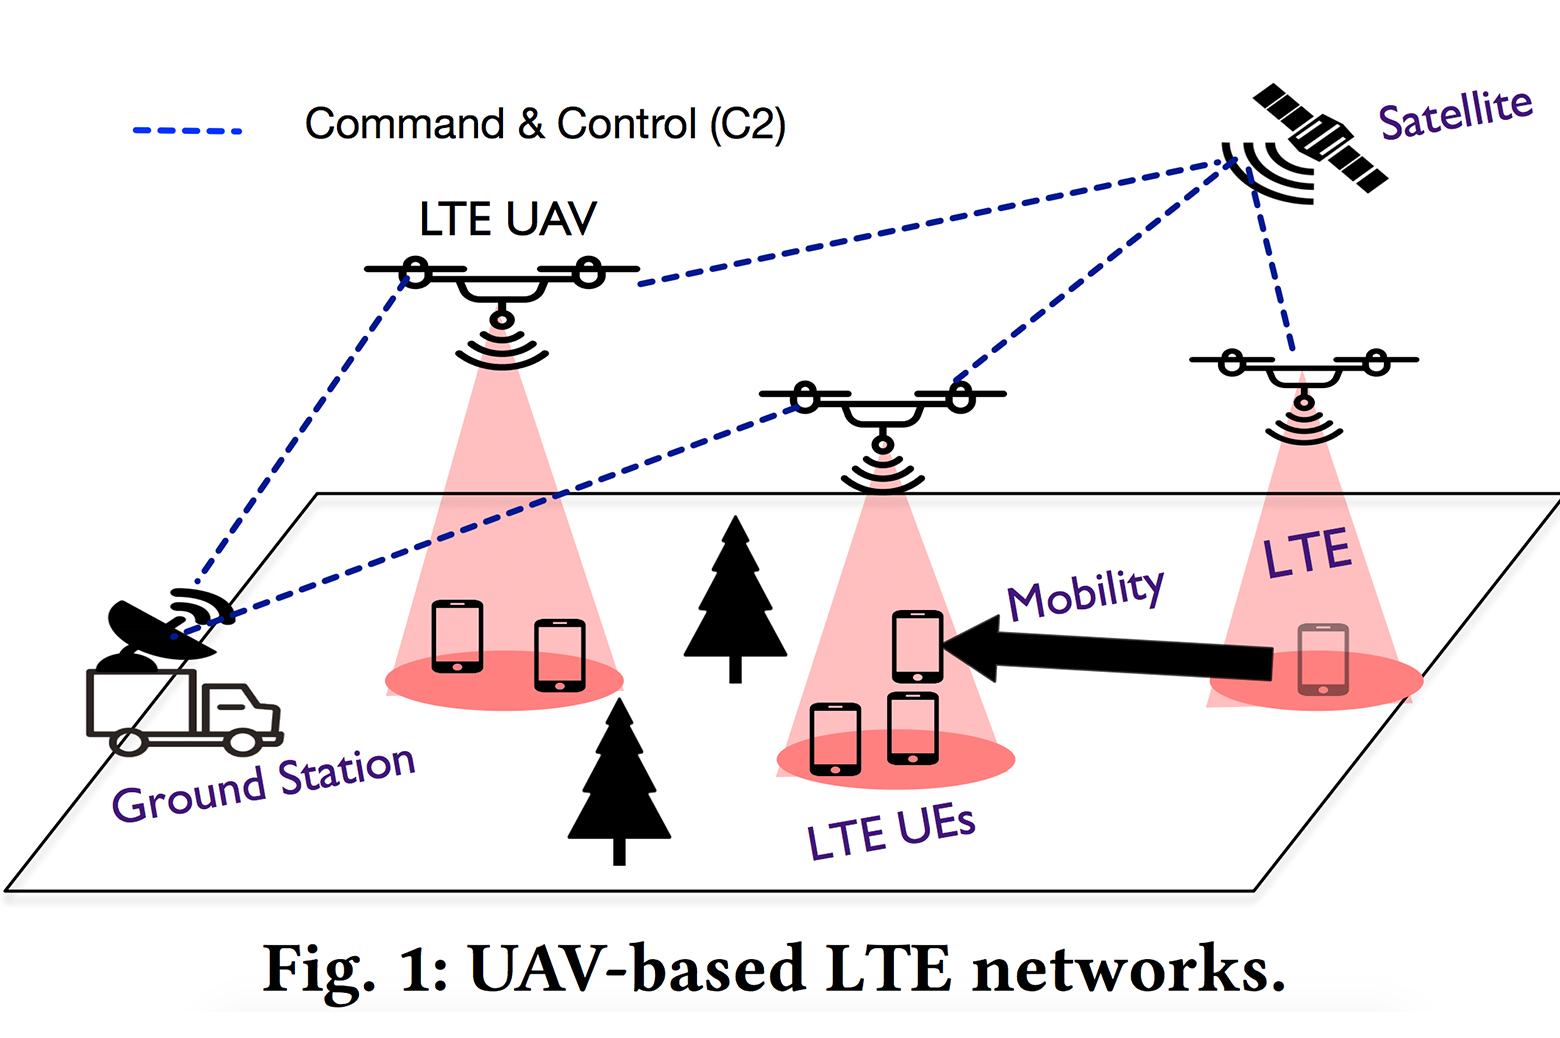
\includegraphics[trim={0 5cm 0 0}, clip, width=1\textwidth, keepaspectratio]{UAV_Integration.jpg}
				\caption{UAV-supported Command \& Control Network \cite{b1}}
			\end{figure}
		\end{column}
	\end{columns}

	\note{From this project, a number of different questions come up. What if we had a massively large dataset?
		When will deep learning beat extreme learning? What could we get out of a real-world test?
		These models were put together relatively quickly as a kind of proof of concept, and more fine tuning may
		yield better results.
		Real world scenarios are also more complex with more than just one UAV and one Base Station.
		Integrating this work into an actual deployment scheme would require more effort.
		Overall, this project shows how edge machine learning can be useful in specific scenarios where UAVs may
		be used for supporting a wireless network.
	}
\end{frame}

\begin{frame}{Future Work}
	\begin{columns}
		\begin{column}{0.5\textwidth}
			\begin{itemize}
				\setlength\itemsep{1em}
				\item Further Model Analysis
				\item AERPAW Experimentation
				\item Iterative Design
			\end{itemize}
		\end{column}
		\begin{column}{0.5\textwidth}
			\begin{figure}
				\centering
				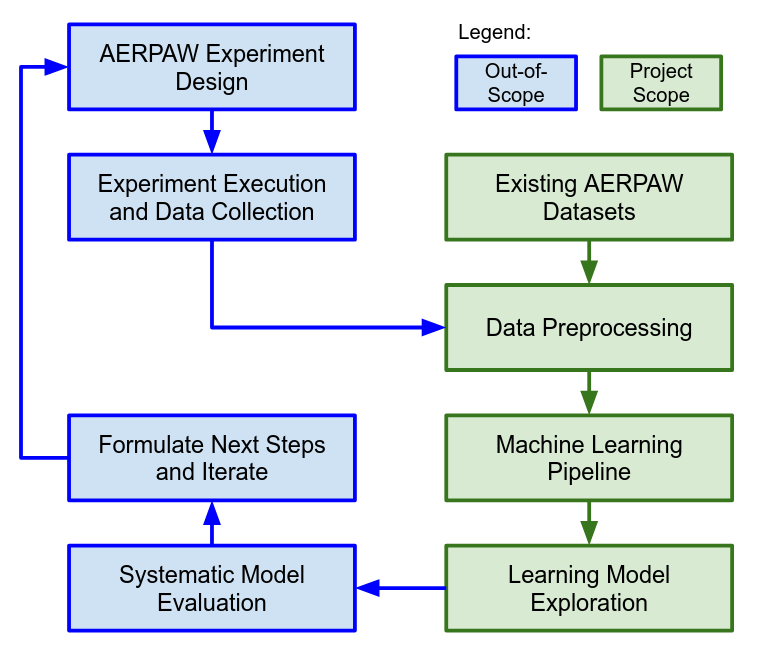
\includegraphics[width=0.9\textwidth, keepaspectratio]{Layout_Flowchart.png}
				\caption{Project Layout Flowchart}
			\end{figure}
		\end{column}
	\end{columns}

	\note{This project not only serves a standalone investigation into deep learning and lightweight
		learning models for UAV radio map modeling, but it will also enable future research into this area.
		This project did not have time to perform a systematic analysis over several different learning models,
		or create an actual AERPAW experiment.
		But this project does give Shadab and Dr. Haihan a better understanding of the research space and
		how they can use their skills to make an impact in this area.
	}
\end{frame}

\begin{frame}
	\centering
	\color{VTMaroon}
	\LARGE
	\textbf{Questions}
\end{frame}

\end{document}
